\chapter{Introduction}
In this work, the design and implementation of a social networking platform for designers of Multi-Cloud applications is presented. In this targeted social networking platform, DevOps~\cite{loukides2012devops} and particularly cloud deployment specialists can benefit from other users' experience and answer design questions such as which is the most cost-effective deployment and which configuration fits their needs. 

DevOps consists of several types of specialists such as programmers, testers, QA staff and specialists from Operations who all use tools for various purposes like building applications, testing, deploying routines, configuration, automation of utilities, tracking and versioning in systems.  
Cloud Deployment Specialists are responsible for migration and configuration of hosted solutions for applications. Furthermore, they have deep industry knowledge about security, auto scaling, storage, load balancers, CDN and everything related to an application's secured hosting and scalability. They communicate with each other and exchange opinions on cloud deployment of applications. Having a repository, where they can find the configurations and the executions data of an application and point to those data, can make their conversation specific and help them come to more concrete conclusions.

This social network targets the cloud deployment specialists and binds all social networking concepts such as personal messaging, groups, new feeds with concepts of application composition and deployment, integrating a repository of cloud applications and infrastructure description based on Cloud Application Modelling and Execution Language (CAMEL)~\cite{paasagedeliverable212}. 

This CAMEL repository means to several benefits to the DevOps community.
Among the range of possible DevOps tasks, the Social Network focuses on selecting the most appropriate deployment
configuration for an application. This is especially challenging in a multi-cloud setting due to the
large diversity of deployment possibilities and tradeoffs. Currently DevOps users work with a small set of
well-understood deployment options, missing opportunities for improving performance, reliability and/or
lower cost. Investigating new options involves time consuming testing over new infrastructures. Discussing
with the community in online social or technical forums may provide insight over deployment options;
however the answer to a hard question often needs to be backed by experimental data that is not readily
available. 

An integrated environment can enrich user interactions with structured references to applications and their components, execution data, and mined knowledge from real deployments. Mined knowledge can be combined with user activity and profiles to provide personalized suggestions and hints.  An improved mode of user interaction is expected to result to stronger incentives for DevOps users to contribute information to the underlying repositories. More content should lead to better quality of mined knowledge, benefiting the DevOps community and providing further incentive for contributions.  The social networking platform designed to be closely integrated with a set of information repositories satisfying the following requirements: 
(R1) handle entire applications rather than just software components; (R2) abstract application structure through software modeling; (R3) capture and analyze application runtime performance. 

Raising the level of abstraction from the components to the whole applications and the analysis of application execution data, can provide answers to many interesting questions of the community and support discussions and arguments with hard data. 
These requirements can provide software developers with strong incentives to contribute, leading to the sustainability and growth of information and derived knowledge in the repository.

The key contributions of this Social Network platform(SNP) are:
\begin{itemize}
\item The SNP binds together all the Social Networking aspects such as friends, new feeds, messages etc. with the engineering aspects of creating and deploying application models.
\item The SNP brings to the light the execution histories of the CAMEL applications, providing to the end users the ability to browse, discus, point and find the information needed for other applications.
\item The SNP use known best practices for both the front end viewing system and the back end scaling system. 
\end{itemize}

This thesis is structured as follows in the~\ref{sec:background} presented the background of application models and the CAMEL repository in the context of PaaSage EU project, in the section~\ref{sec:related} described the previous work based to Social Networking Platforms. In the chapter~\ref{chap:implementation}, the system implementation of the Social Network is described and the chapter~\ref{chapt:evaluation} evaluates the implemented system.
%\section{Motivation}

\section{Background}
\label{sec:background}
Application models inside social network platform are described in CAMEL. CAMEL integrates various domain-specific languages (DSLs). These DSLs cover a wealth of aspects of specification and execution of multi-cloud applications like CloudML, Scalability rules, WS Agreement, Saloon and Historical Execution Data. 
CloudML~\cite{FerryRossiniCMS13} is a recent approach that focuses on the provisioning and deployment of multi-cloud applications, is built upon MDE techniques and methods, and provides a models@run-time~\cite{models-runtime} environment for enacting the provisioning.  WS Agreement~\cite{andrieux2007web} is a Web Services protocol for establishing agreement between two parties, such as between a service provider and customer. Saloon ~\cite{quinton2013towards} is an approach that uses models to represent clouds variability, as well as ontologies to describe the heterogeneous aspect of the cloud ecosystem. The CAMEL model couple together all those DSLs as shown in figure~\ref{fig:dsls}.

CAMEL is using the Eclipse Modelling Framework (EMF)~\cite{steinberg2008emf} on top of the Connected Data Objects (CDO)~\cite{cdomodel}. Application Models are persisted on the CDO repository. EMF is used as a building tool for the application models. CAMEL model specification described in XMI format (XML Metadata Interchange) consisting the core system of CAMEL and provides tools that enable viewing and command-based or tree-based editing of the application models.

\begin{figure}[h]
	\caption{CAMEL DSLs.}
	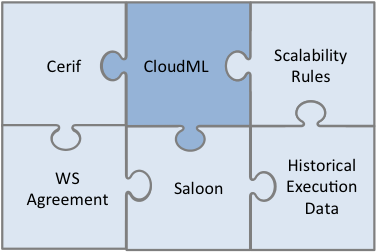
\includegraphics[width=0.6\textwidth,natwidth=200,natheight=150]{./fig/dsl.png}
	\centering
	\label{fig:dsls}
\end{figure}

The Social Network Platform is part of the PaaSage EU Project~\cite{paasage}.
The PaaSage perspective is to be a tool for a Cloud Deployment Specialist to leverage the complex task of deploying an application to the Clouds. The Cloud Deployment specialist usually could learn the interface and features of only one Cloud provider, but it would be very costly and time consuming to leverage the development to many providers. It is a real challenge to orchestrate the simultaneous deployment to many different Clouds at the same time. The main objective of PaaSage is to assist the developer to deal with difficult deployment scenarios through automatic cloud deployment. In order to satisfy this, several components are included to the PaaSage ecosystem. The Profiler components read the CAMEL models and convert them into a constraint programming model by defining the variables of the model, their domains, and the constraints that must be satisfied by the deployment. Also, the Profiler checks all constraints of the CAMEL model and sets the domains of the variables accordingly. The reasoning component analyses the model and finds how deployment candidates should be evaluated. Once a solution has been found, the reasoning component converts the model to Cloud Provider Specific Models (CPSM) for the providers involved in the proposed deployment. The adapter component takes the CPSMs, produces and validates a configuration plan, and sends this plan to the execution ware. The execution ware receives the deployment plan from the adapter and enacts the deployment of the application on the selected providers. Furthermore, the execution ware interacts with the Cloud providers, acquires the virtual machines, configures them and launches the user application on the set of virtual machines. Once the machines are running, the execution ware collects sensor data for the running application, triggering re-configurations if necessary.
The PaaSage Social Network brings to the end users a friendly interface to interact with those components.


%\section{Methodology}

%\section{Other section}
